\chapter{Background}

The classical approach to extract useful information from an image has been to find mathematical definitions for features that describe the information. The features could, for example, be lines, circles, or edges. 
Circles can be used to find coins, where the diameter denotes the value. Lines can be used to find how many fenceposts are in a fence. Traditional mathematical models include the Hough Transform~\cite{houghTransform} for detecting lines or circles, the Sobel operator to detect gradients, and in return, edges, or the Gray Level Co-occurrence Matrix for detecting texture features. 
In common for all these methods is that they are well defined, and find precisely \emph{one} type of feature that was previously specified. 
At a higher level, hand-crafted feature descriptors have been made. They look for a specific set of features in an image to identify unique locations. Some well-known examples are the SIFT~\cite{sift1999Lowe}, SURF~\cite{surf2006Bay} and ORB~\cite{orb2011Rublee} feature descriptors. They have been used successfully in applications such as combining images into panoramas or combining different views to a 3D model, also known as Structure from motion~\cite{sfm1979ullman}.

Hand-crafted features have also been used in machine learning scenarios. As an example, Haar-like features were demonstrated to efficiently find faces in \cite{haarcascade}. Here, the machine learning model decided which of a given set of features to use to classify whether the frame contained a face or not. In using both the Sobel operator and using Haar-like features, a filter is passed over the image. In the case of the Sobel operator, this is an actual convolution of the image with the filter. This is the intuition that is used in Convolutional Neural Networks, discussed next.

\section{Convolutional Neural Networks}
Instead of using hand-crafted features, \gls{cnn}s \emph{define} the features they use \emph{when they are trained}. 

\gls{cnn}s are widely used in image classification tasks because they look at a collection of spatially connected pixels. This means \gls{cnn}s are robust to the placement of the object in the frame, and even partial occlusions.

\section{Pose Estimation}
Much research has been done in estimating human pose in two dimensions, as quite large datasets have been made, such as the MPII, or the Human 3.6M datasets \cite{andriluka14cvpr,h36m_pami}.

There have been two ways of finding human pose in an image. One is a top-down approach, where a number of persons first are found in the image, and advanced algorithms have refined their pose after finding key features.
The other is to find the key features for the whole image, then build up the instances of people.

In \cite{cao2017realtime}, two \emph{cnn}s are used to estimate human pose. One of the networks produces a \emph{confidence map} for each joint. Each pixel in the confidence map contains the probability, or confidence, that the pixel is part of a person's joint. The other creates \gls{paf}s, which is a map of vectors pointing in the direction of one of \emph{M} limbs. \footnote{This work will stick to the convention of using the term \emph{limb} to describe any \emph{connection between any pair of body landmarks}. The body landmarks will be termed \emph{joints}.} These maps are assembled by bipartite matching to create the 2D skeletons observed in the scene.


\begin{figure}[h]
  \begin{subfigure}[t]{0.24\textwidth}
    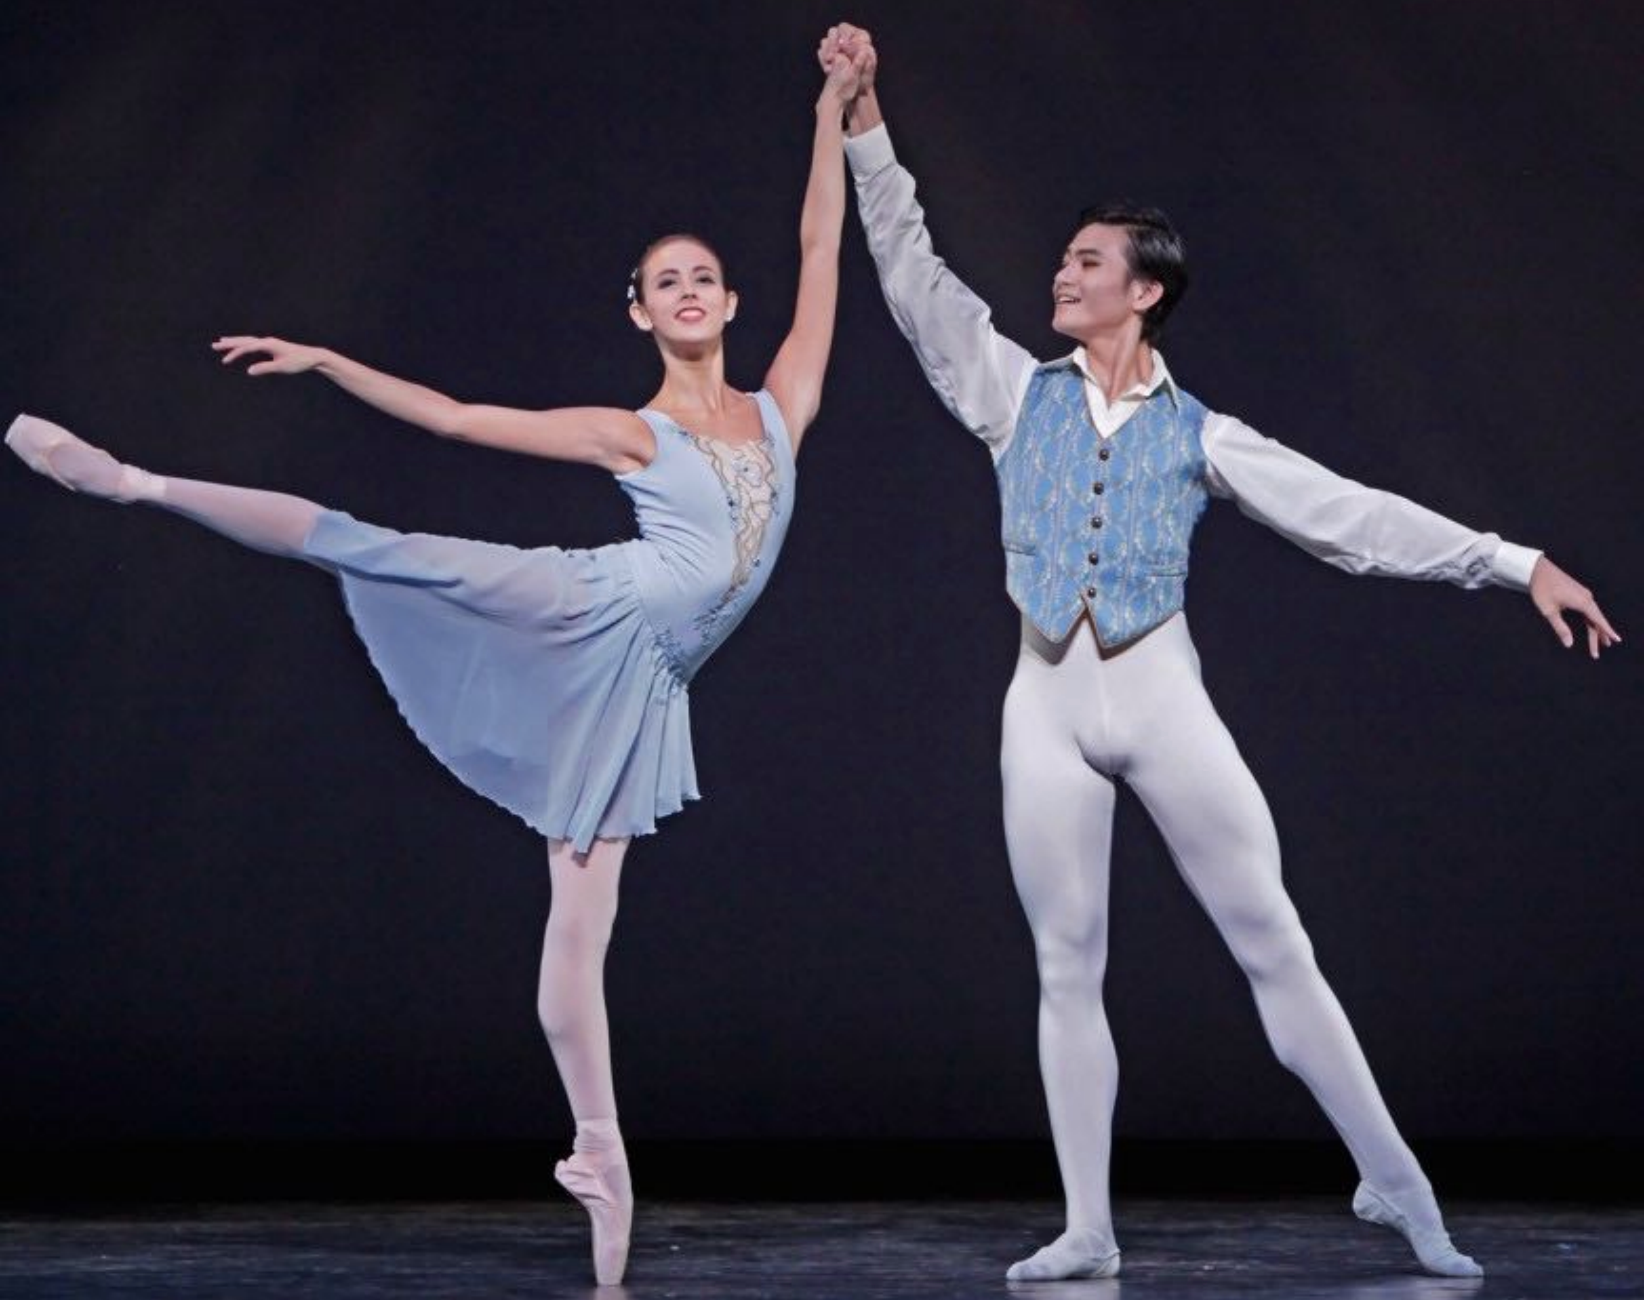
\includegraphics[width=1\linewidth]{img/openpose_pipeline_a}
    \caption{Input Image}
    \label{fig:oppA}
  \end{subfigure}%
  ~
  \begin{subfigure}[b]{0.24\textwidth}
    \begin{subfigure}{1\textwidth}
      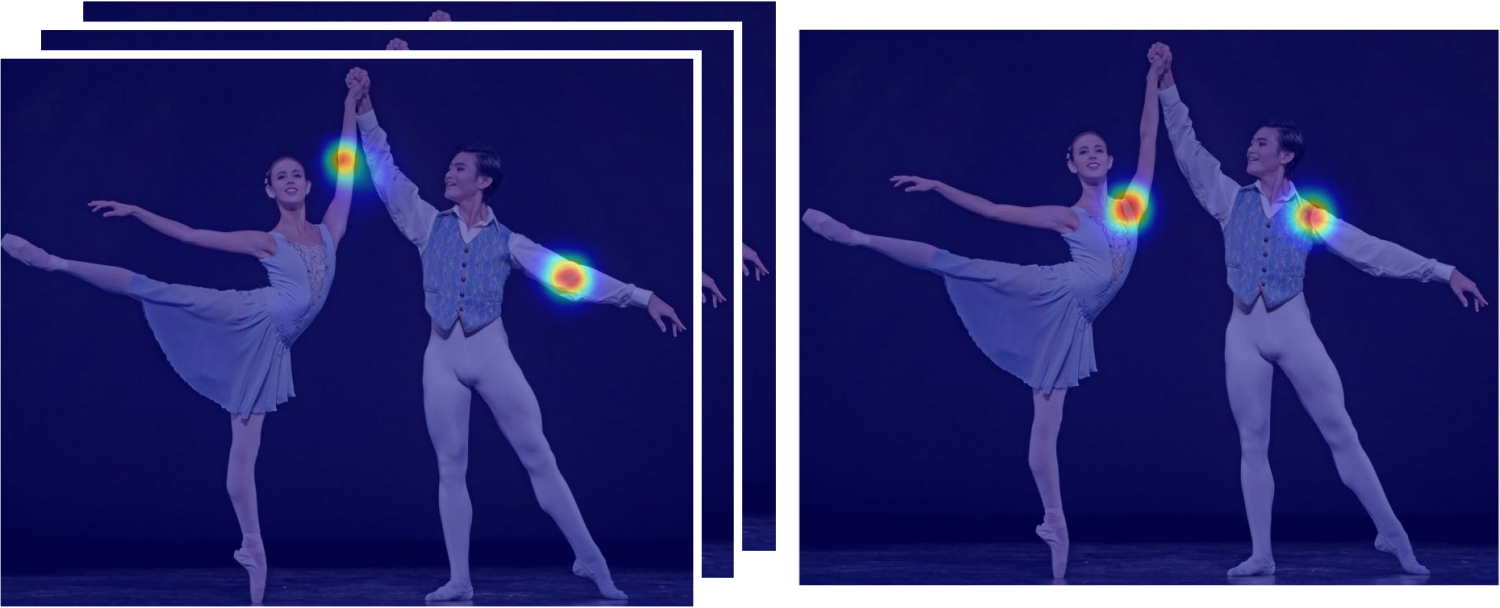
\includegraphics[width=1\linewidth]{img/openpose_pipeline_b}
      \caption{Part Confidence Maps}
      \label{fig:oppB}
    \end{subfigure}
    
    \begin{subfigure}{1\textwidth}
      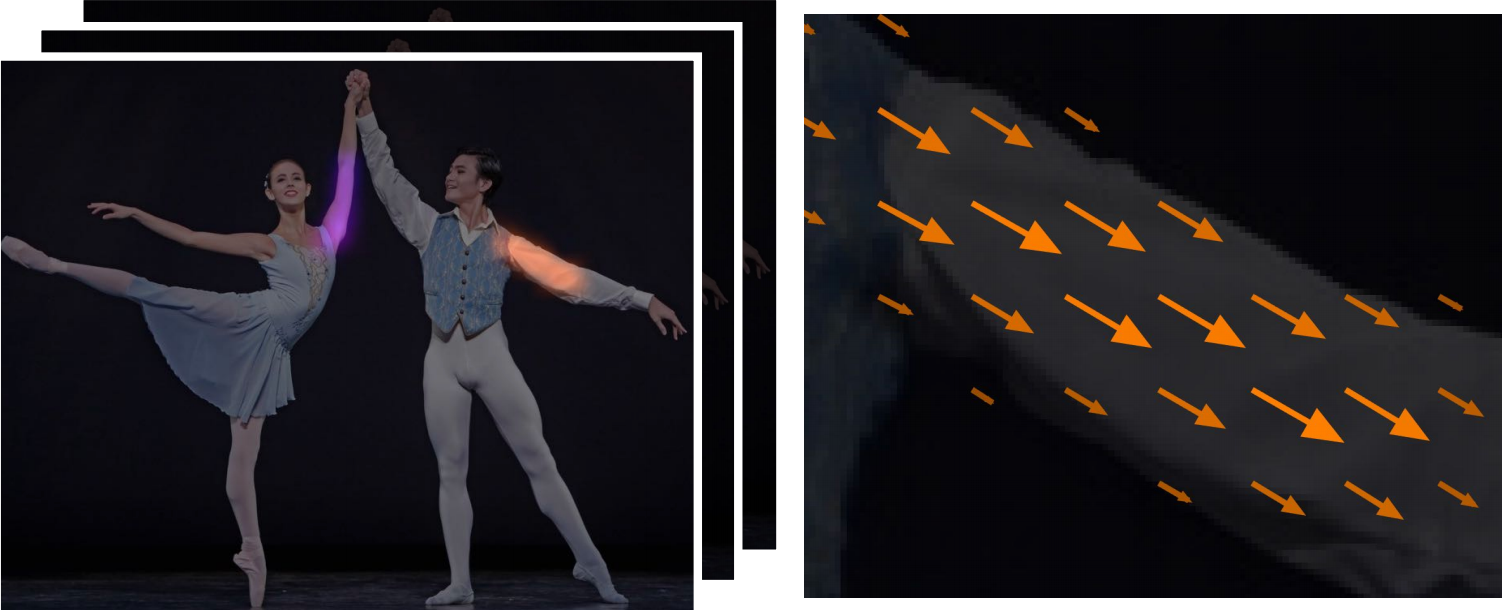
\includegraphics[width=1\linewidth]{img/openpose_pipeline_c}
      \caption{Part Affinity Fields}
      \label{fig:oppC}
    \end{subfigure}
  \end{subfigure}%
  ~
  \begin{subfigure}[t]{0.24\textwidth}
    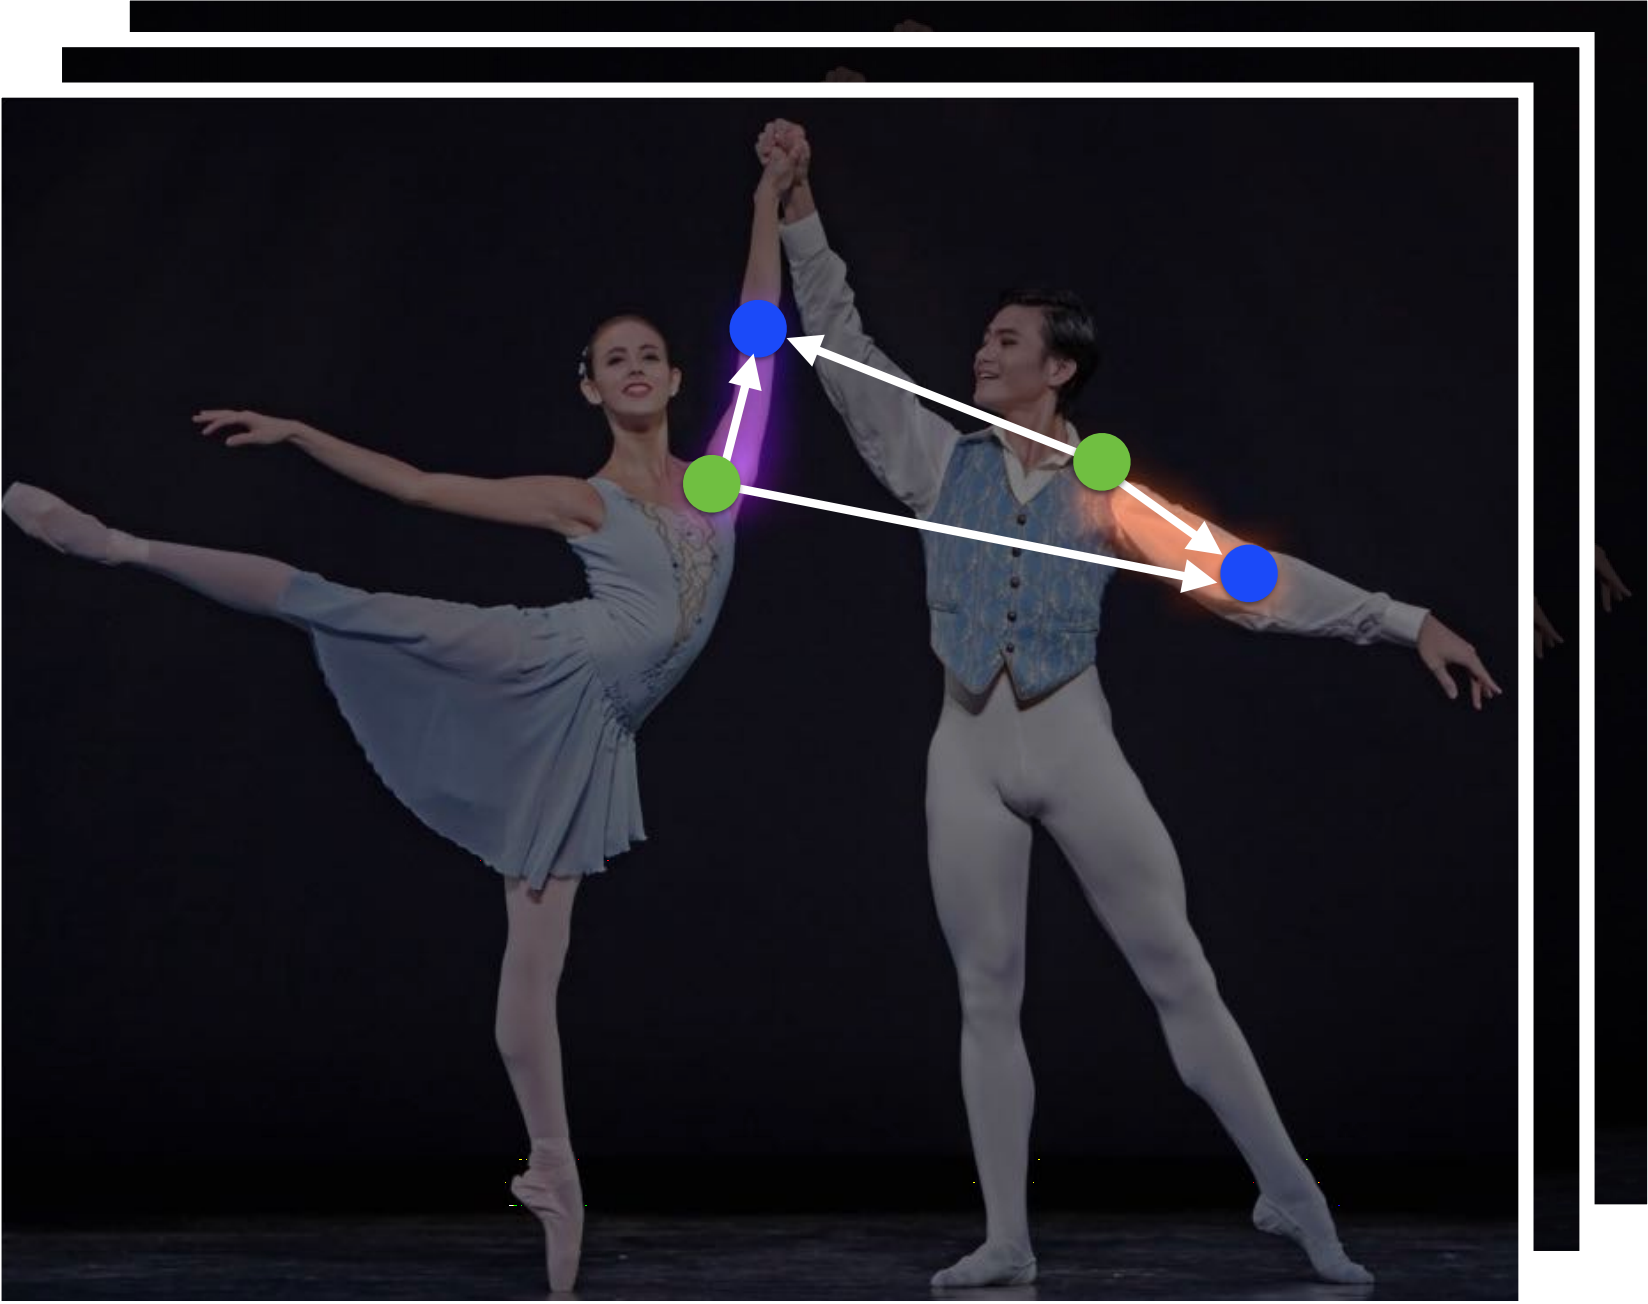
\includegraphics[width=1\linewidth]{img/openpose_pipeline_d}
    \caption{Bipartite Matching}
    \label{fig:oppD}
  \end{subfigure}%
  ~
  \begin{subfigure}[t]{0.24\textwidth}
    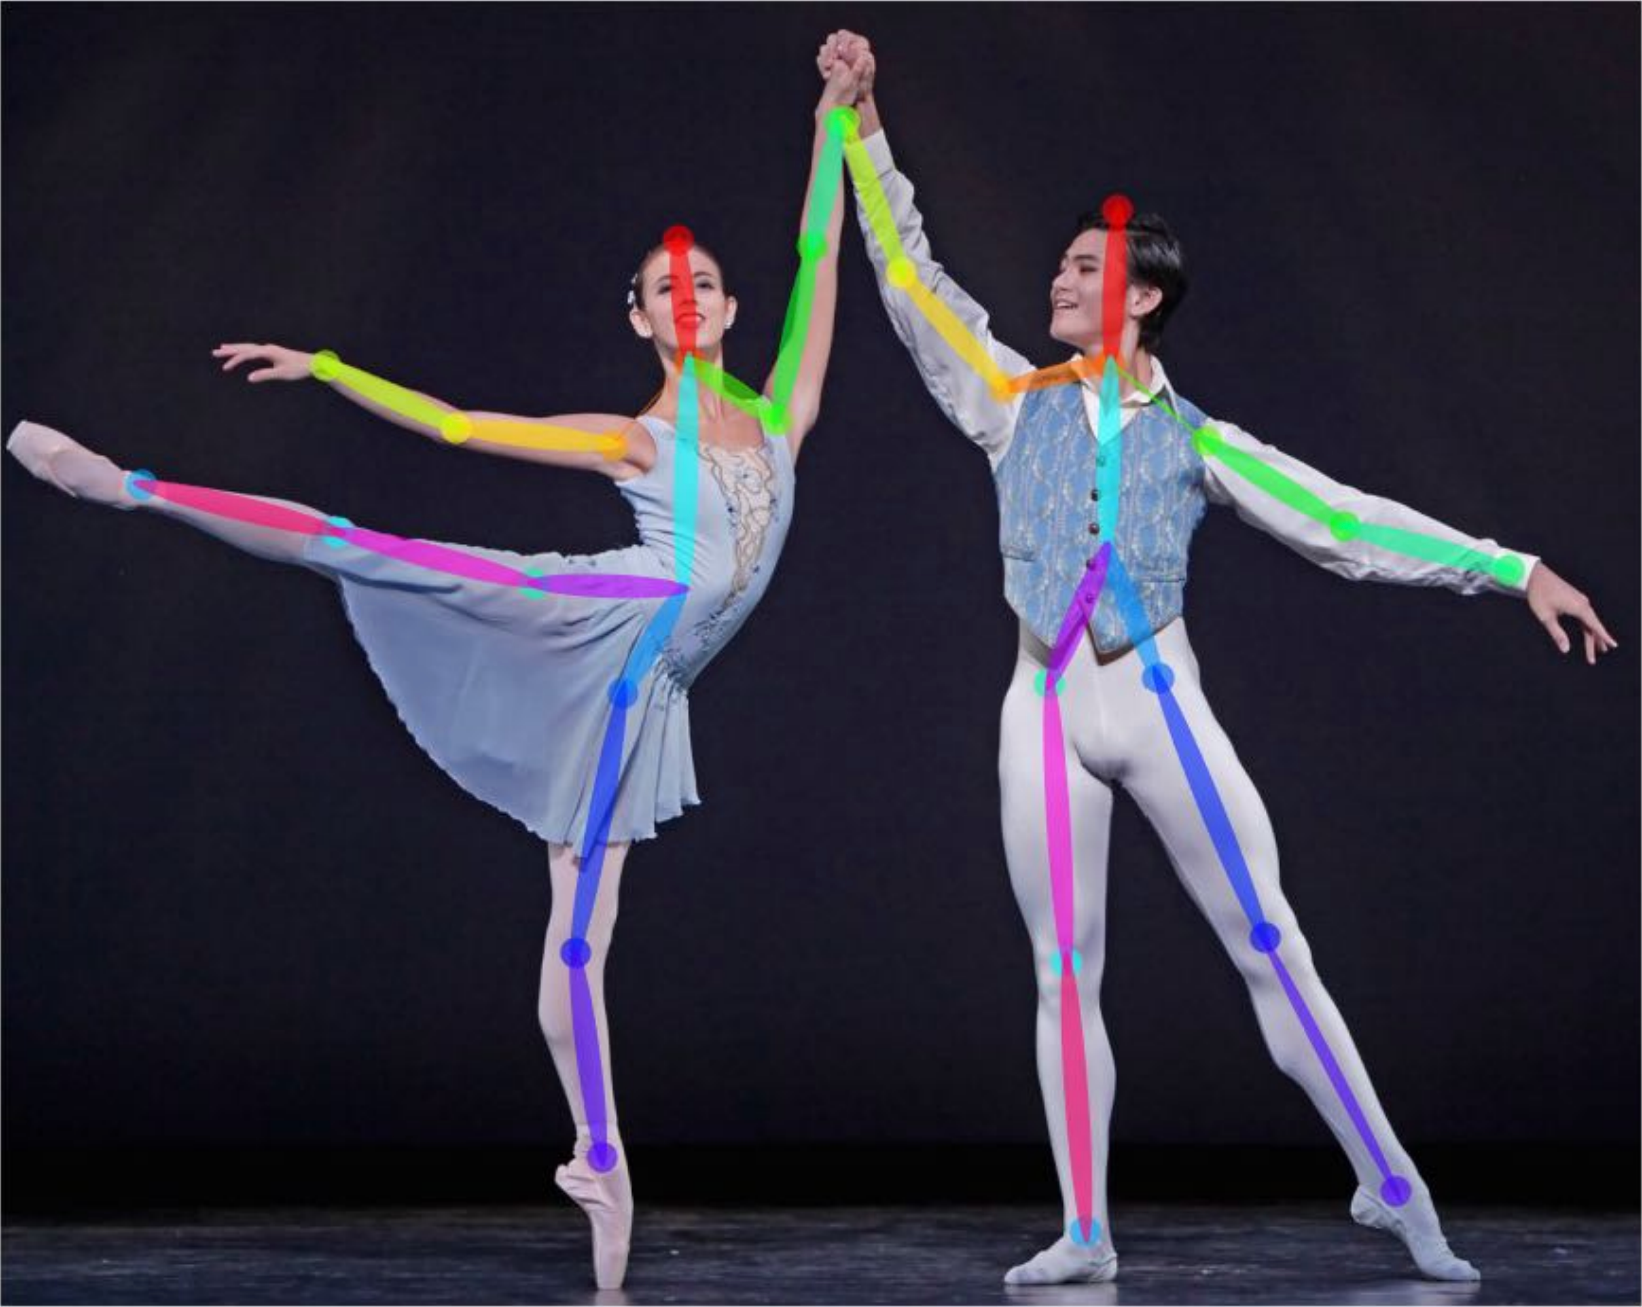
\includegraphics[width=1\linewidth]{img/openpose_pipeline_e}
    \caption{Parsing Results}
    \label{fig:oppE}
  \end{subfigure}
  \caption[OpenPose pipeline]{The pipeline described in \cite{cao2017realtime}. The input image \ref{fig:oppA} is fed into the two networks, which produce joint detections in confidence maps \ref{fig:oppB} and PAFs  \ref{fig:oppC}. Bipartite matching is performed in \ref{fig:oppD}, to determine which detected joints should be connected by a limb. \ref{fig:oppE} shows the finished results.}
  \label{fig:openpose_pipeline}
\end{figure}

Using the method described in \cite{cao2017realtime}, no information is given for joints that are not accurately detected. If, for example, an extremity is occluded together with half of the connecting limb, the extremity will not be part of the output skeleton, even if the joint could be extrapolated from the parts of the limb that is visible.
This is also true for undetected joints in the middle of a joint-chain. The joint could be extrapolated using the surrounding joints. The problem with joint-extrapolation happens because of the bipartite matching, which does not work if any joint is missing.
